\chapter{Entanglement Entropy in de Sitter space}

\begin{comment}
  \section{Euclidean vacuum mode functions for a scalar field on open de Sitter space\cite{10}}

  低密度で負の曲率宇宙を予測するoneバブルのinflationalな宇宙シナリオの最近の研究によって動機づけられ、双曲線タイムスライスによって構成されるドジッター時空のopen chartにおけるのスカラー場のユークリッド真空モード関数を調べる。

  初期の状態のすべての情報を失うほど、初期のinflation時代が長過ぎてはならないので、open inflationalな宇宙の可能性を考えるとき,インフレーションを引き起こすためのinflaton場の量子揺らぎの初期条件に関する問題に直面する.

  false真空の量子減衰によって,指数関数的に拡大するfalse真空宇宙でオープンな宇宙が生成されるワンバブルのシナリオでは、初期状態はドジッター不変のユークリッド真空は正当化される。ここでは、ユークリッドの真空モード関数とは、任意の質量と曲率結合を持つスカラー場のオープンチャートに関して示す。

  興味深いことに、無次元masslessのコンフォーマルスカラーに対応する臨界値よりも小さな有効質量を持つスカラー場のために、オープンチャートの時間一定面の超曲面上で平方積分可能ではない離散モードのセットが現れる
  \subsection{Introduction}
  最近の観測結果からわかることは,宇宙の曲率は,負極率であることが示唆されている,一つのConsistentなpen宇宙の出現のシナリオに,擬真空が支配的な宇宙の加速度膨張が上げられる.このideaは,Gottによって初めて提唱された.\cite{11}スタンダードなinflationシナリオの枠組みでは,horizon問題は,空間の急激な膨張によって解決される.平坦チャートの晴れる大きさは,はじめhorizon程度の大きさだあったが,宇宙の急激の膨張で膨張し,現在のわれわのhorizonサイズは,その平坦チャートの中にいることで平坦性問題がhorizon問題と同時に解決された.したがって,現在の我々のいる宇宙の曲率は,必然的に膨張とともに減少していくことになる,これは,open universeを考える上で問題になる,
  一方,擬真空においてde Sitter時空で記述されるバブルが生成されたと考えると,トンネル効果によってEuclidianな対称性O(4)を持つ時空から生成されるのでO(3,1)対称性を持つことになる,この時,ユークリッド時空なので因果関係などはなくhorizon問題は,解決される,

  \textcolor{red}{O(4)とかO(3,1)あたりがわかっていない
  de Sitter時空にO(3,1)があるのか,de Sitteとは何か.つまり,Minkowsikiとどう違うのか.
  メトリックは違うが,対称性に関しては同じ感じがするが}

  もし,バブル生成が起こってから,真空のエネルギーが宇宙のエネルギーのうちう優勢な要素に永遠にならなければ,曲率のエネルギーがずっと優勢になり,観測されているようにFRW universeが結論付ける,\textcolor{red}{ここら変の議論が実際にペンを動かして確かめる必要がる,}Bigbangやそれに伴うhotなeraが実現されない.そうすると,エントロピーが生成される過程が生まれないために,Entropy Problem\footnote{There exists the 'entropy problem' of the early universe, that is, why did the universe begin with an extremely low entropy and how did it evolve into such high entropy at late times? }が解決されないことになる,そこで,secondary inflationがバブル内で起きることを要求する.このモデルが,スタンダードなinflationシナリオと本質的に異なるポイントは,secondary inflation開始時の曲率程度のスケールのhorizonサイズのpatchが,現在の我々のhorizonサイズよりはるかに大きくならない可能性がある,

   これは、secondary inflationの開始時の宇宙の量子状態の記憶は消去されず、観測された大規模な温度と密度の変動に直接影響を与えることを意味することになる,\textcolor{red}{ここら辺の量子状態の記録が消える消えないの議論がわからない,また,なぜpatchの大きさがそれに関係し,そのスケールが曲率のスケールくらいなどと予測されているのか.仮説としては,secondary inflationの場合は,宇宙の膨張が抑えられて,現在観測している我々のデータに,secondary inflation前の量子状態が影響するという意味なのかなって感じ.}

   したがって,我々は,バブル内のsecondary inflation時におけるinflaton場について色々と調べる必要が出てくる.これに関する先行研究は,様々に行われていて,O(4)におけるトンネリング効果に関する公式などが開発された.これまでの研究はすべて、一般的な状況に実際に適用可能な量子状態を調べる技術はまだないという意味ではかなり正式なレベルにとどまっていた.(rather practical level to general situations)

  しかし,それは,拡張され\cite{12},この論文ではさらに重力を入れて考え他場合について議論する.

  第1のステップとして、重力のバックグラウンド反応が無視され、バックグラウンドメトリックがde Sitter空間に固定される場合を考える。次に、bubble内部の時空は、空間が開いているde Sitter空間のチャートによって記述され、inflaton場は、空間的に開いた時間スライスの超曲面で一定の値をとる。さらに、バブル核形成を引き起こすトンネル場がinflaton場$\phi$と相互作用しない場合、$\phi$の量子状態はトンネリングプロセスの影響を全く受けない。次に、トンネリング前の$\phi$の量子状態がユークリッド真空であることを前提とする。これは先の擬真空膨張が十分に長く続く場合には良い近似であるはずであるが、bubble内部の量子状態はそのままである。そこで,de Sitter空間のオープンチャートでモード関数によって量子状態を記述する必要があります。openチャートでユークリッド真空モード関数を得る方法が分かったら、トンネルを起こす場との結合によって$\phi$の質量が時間的に変化する場合や幾何が後の段階で正確なde Sitter空間から逸脱した場合に拡張するのはかなり簡単にになる,

  ちなみに,de Sitterの場合でもflat chartとclosed chartでは先行研究がある, \cite{13}とかT.S.
  Bunch and P.C. Davies, Proc. R. Soc. London, Ser. A 60, 117 (1978), B. Allen, Phys. Rev. D 37, 2078 (1988).
\end{comment}












\section{Set Up}
\textcolor{red}{もう一度構成から書き直しをする.足りないところは手書きノート見ながら埋める.}
この章では,まず,これからどのような設定でエンタングルメントエントロピーを求めるかを決め,そのエンタングルメントエントロピーをどのようなステップで求めるかを述べる.

はじめに我々の目標は,de Sitter時空の真空の大局的な相関\footnote{エンタングルメントエントロピーは,大局的な相関である.普段CMBなどで考えている相関は,局所的な複数の点の壮観である.エンタングルメントエントロピーの相関は,領域同士の相関である.}を求めることである.この真空の相関は,宇宙が膨張する時に生じたものである.de Sitter時空を考える理由は,初期宇宙がde Sitter時空に近似できることから初期宇宙で生じたエンタングルメントエントロピーを評価するのに適しているからである.
\subsubsection{de Sitter時空におけるevent Horizon}
今,時刻$t=0$に$x=0$地点にいるObserverを考える,宇宙が膨張しているので,十分遠方からの光は観測できないと推測される.そこで,このObserverに届く情報はObserverからどの距離までにあるのかについて求める.情報が届かなくなる境界のことをよくEvent Horizonと呼ぶ.宇宙の中で最速なのは光であるので,光が無限の未来にObserverに到達するような場合の,光源のある場所がちょうどEvent Horizonとなる.したがって,Observerからその光源までの距離は,
\begin{align}
  l_{ds}&=\int_{null}|d\bvec{x}|\\
  &=\int^{\infty}_{t}\frac{dt^{\prime}}{a(t^{\prime})}
\end{align}
となる,1行目から二行目の変形は,nullは$|d\bvec{x}|=d\eta=\dfrac{dt^{\prime}}{a(t)}$であることを用いた.(a)の図における,メトリックは
\begin{align}
ds^2=dt^2-e^{2H_{dS}t}d\bvec{x}^2
\end{align}
()式で表せるので,$a(t)=e^{H_{dS}}$である.ゆえに,
\begin{align}
l_{dS}=\frac{1}{H_{dS}}
\end{align}
となる.
$dt=e^{H_{ds}t}d\eta$を用いてconformal time$\eta$を導入する.すると,
\begin{align}
\eta=-\frac{e^{-H_{ds}t}}{H_{ds}}
\end{align}
であるので,
\begin{align}
e^{-H_{ds}t}=-H_{ds}\eta
\end{align}
を用いると,メトリックはもっと簡単に,
\begin{align}
ds^2=\frac{1}{(H_{ds}\eta)^2}(-d\eta^2+dx^2+dy^2+dz^2)
\end{align}

\section{de Sitter時空の対称性}
4次元de Sitter時空は5次元Minkowski時空,
\begin{align}
  \label{EDS}
  ds^2_{5}=-dX_0^2+dX^2_{1}+dX^2_{2}++dX^2_{3}++dX^2_{4}
\end{align}
に埋め込まれた双曲面,
\begin{align}
  +X_0^2-X_1^2-X_2^2-X_3^2-X_4^2=R_{ds}^2=H^{-2}
\end{align}
によって表現される.この埋め込みによって得られるde Sitter時空のFlat Chartは,
新しい座標系($\tau,x_{i}$)を用意することで実現される.新旧の座標の関係は,次で与える.
\begin{align}
  X_{0}=&\frac{1}{2H}(H\eta-\frac{1}{H\eta})-\frac{1}{2}\frac{x_i^2}{\eta}\\
  X_{i}=&\frac{x_i}{H\eta}\\
  X_{4}=&-\frac{1}{2H}(H\eta+\frac{1}{H\eta})+\frac{1}{2}\frac{x_i^2}{\eta}
\end{align}
ただし,先にも述べたように$\eta<0$である.
この変換の下で,メトリック(\ref{EDS})式は,
\begin{align}
  ds^{2}=\frac{1}{H^2\eta^2}(-d\eta^2+dx_{i}^2)
\end{align}
と,Flat chartのメトリックになる,ここで,このchartが覆っている領域は,上の対応関係から,$X_{0}+X_{4}=-\frac{1}{2H^2\eta}>0$であるので,図\ref{vchart}のFlat Chartのように全体の斜め半分のみを覆うことがわかる.ここで,$\eta\to 0$の極限では,この座標の対応は,
\begin{align}
  X_{0}=&-\frac{1}{2H^2\eta}-\frac{1}{2}\frac{x_i^2}{\eta}\\
  X_{i}=&\frac{x_i}{H\eta}\\
  X_{4}=&-\frac{1}{2H^2\eta}+\frac{1}{2}\frac{x_i^2}{\eta}
\end{align}
となり,これは近似的に,
\begin{align}
  -X_{0}^2+X_{i}^2+X_{4}^2=0
\end{align}
満たす.すなわち,$\eta\to0$の極限では,時空は近似的に,
\begin{align}
  X_{A}\to\lambda X_{A}
\end{align}
のscale変換の下で不変である.今,$X_{A}$は,$\frac{1}{\eta}$の一次関数で関数であらわせれているから,
このこの対称性から,$\eta$がrescalingできることになる.さらに,エントロピーを評価する$\eta=$一定面上でのメトリックは,
\begin{align}
  ds^2_{\eta\to0}=\frac{dx^2_{i}}{H^2\eta^2}
\end{align}
となるので,時空は,$\eta\to\lambda\eta$と同時に$x_{i}\to\lambda x_{i}$とする変換の下でも不変である.
\begin{itemize}
  \item{時空は,$\eta\to\lambda\eta$とする変換の下でも不変}
  \item{時空は,$\eta\to\lambda\eta$と同時に$x_{i}\to\lambda x_{i}$とする変換の下で不変}
\end{itemize}
以上のことから,$\eta\to0$の極限では,時空に$x_{i}\to\lambda x_{i}$の変換の下での対称性があることがわかる.したがって,de Sitter時空におけるエンタングルメントエントロピーにおける時間に依存しないLong-ange部分は,この空間方向のリスケールによって不変である.すなわち,Entangle Surfaceはこのcomformal trasformationでGlobal chart(Flat chart)における時間一定面のSlice($S^3$)のちょうど真ん中の$S^2$面になるように取ることができる.この事実から,我々は,Open ChartにおけるR,L領域とentangle serfaceの中と外を対応付けられる.
そこで,これ以降は,Flat chartにおけるEntangle Surfaceの中と外の相関を求めるために,Open chartのR,L領域のエンタングルメントについて考える.さらに,Open chartのR,L領域のエンタングルメントについて考えるために,de Sitter時空におけるOpen chartの場の理論について勉強する必要がある.


  \begin{figure}[H]
    \begin{center}
    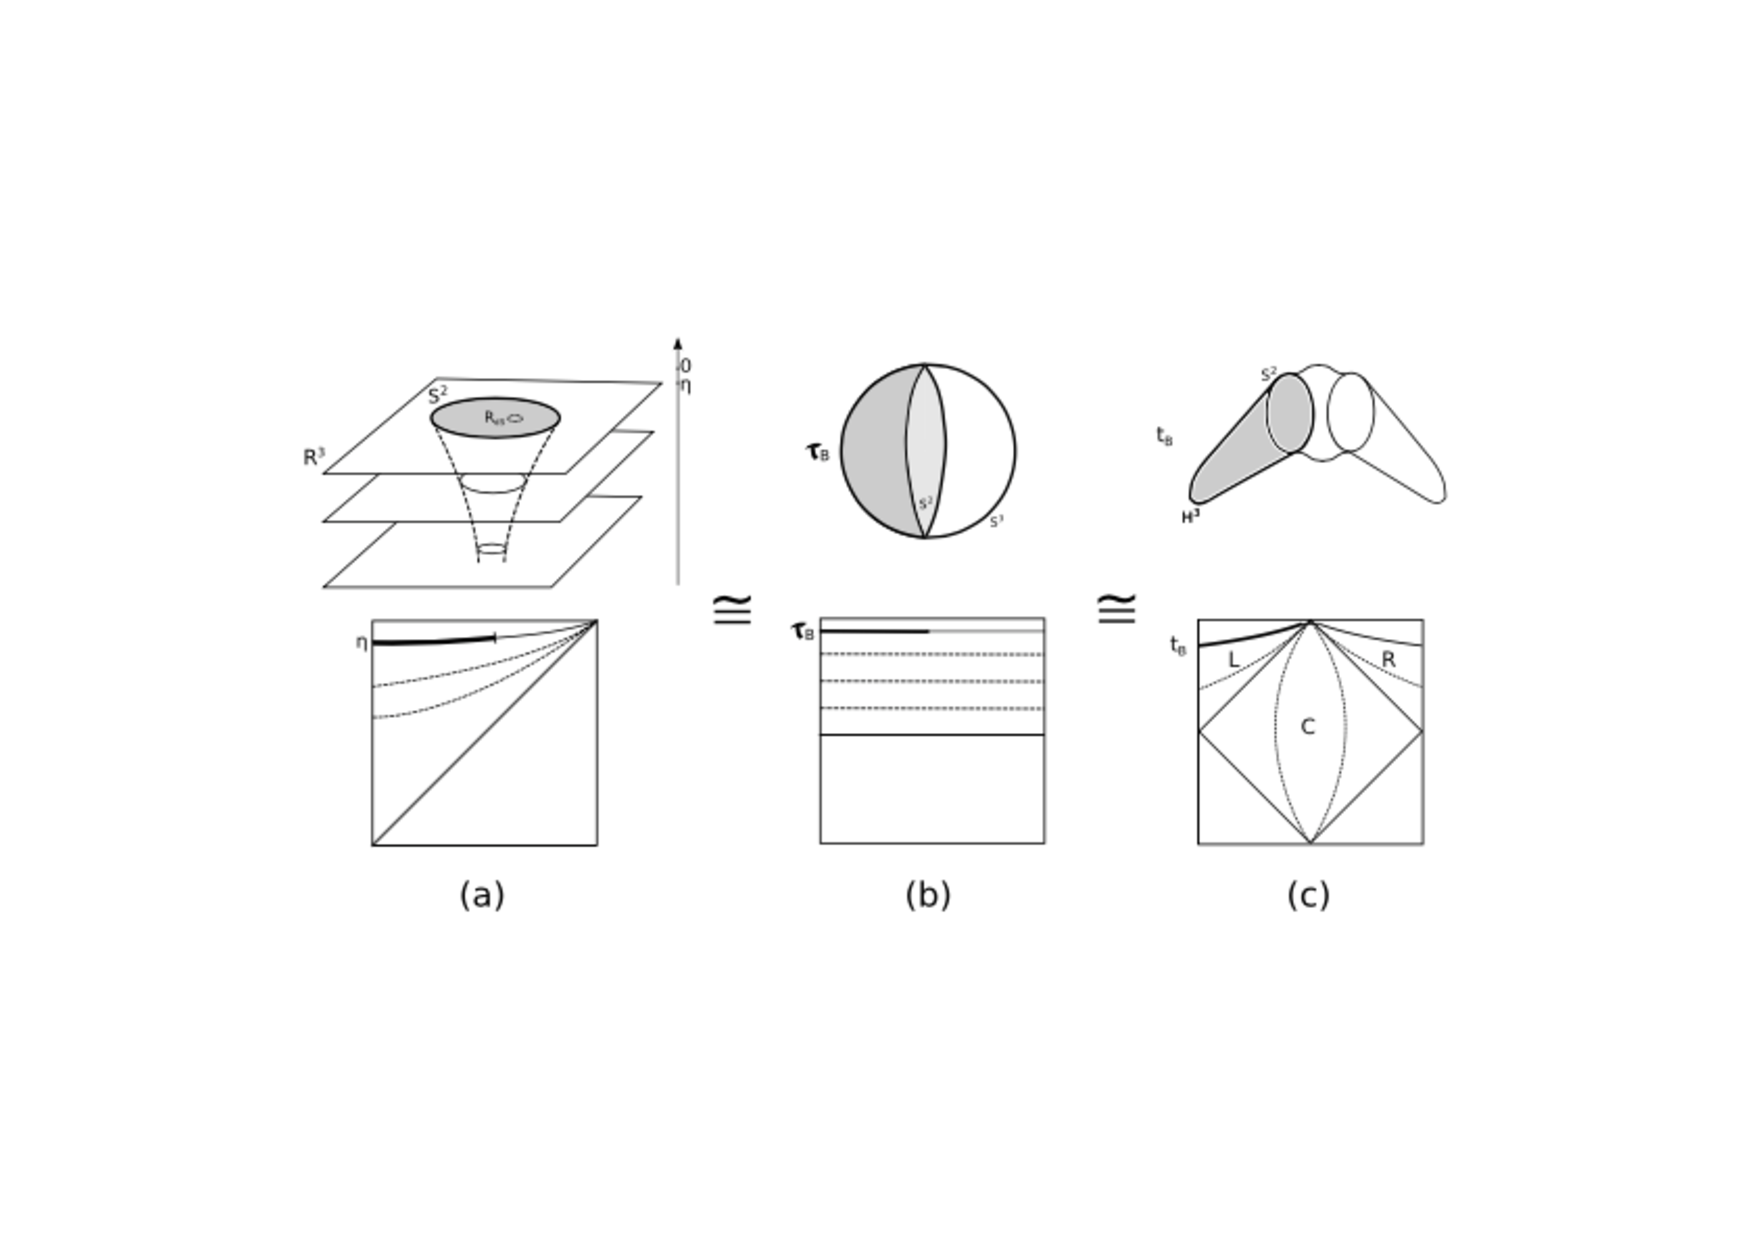
\includegraphics[width=8cm,angle=270]{de.pdf}
    \caption{title}
    \end{center}
  \end{figure}

  \begin{figure}[H]
    \begin{center}
    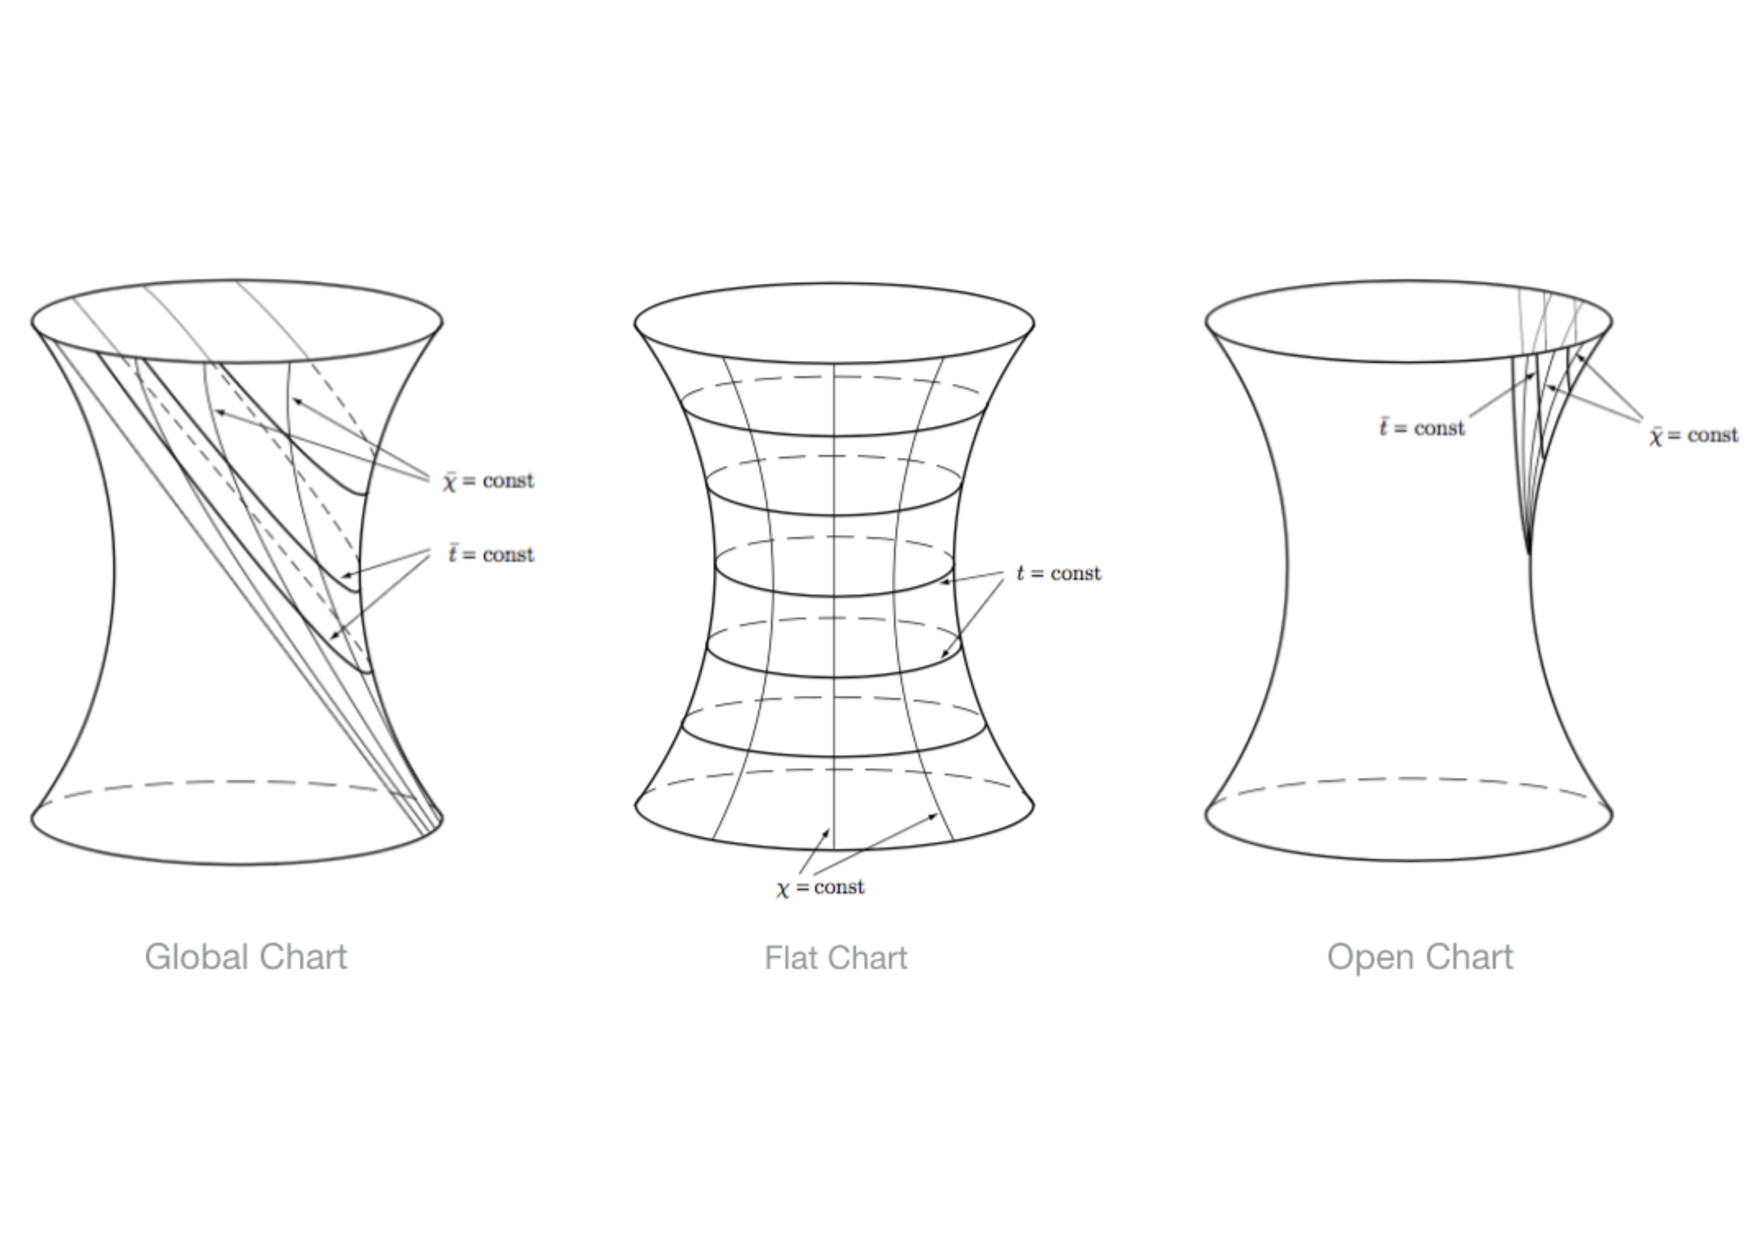
\includegraphics[width=6cm,angle=270]{Web.pdf}
    \caption{de Sitter spaceの様々なChat}
    \label{vchart}
    \end{center}
  \end{figure}

\section{Scalar Field on Open de Sitter Space}
ここでは,de Sitter時空のopen chartでのスカラー場のモード展開に浮いて議論する,
まずはじめに,あとで波動関数の規格化を行う際に,R,L,C領域がそれぞれどのような関係性になっているかについて知る必要がある.(具体的には,解析接続で繋がっていることを用いて,de Sitter space全体に渡ってCauchy surfaceを定義して規格化を行う.)
\subsubsection{Global Chart}
\textcolor{red}{まずはじめにFlat chartのメトリックがどのような形をしているのかそれぞれの領域のメトリックを見せる.次にそのメトリックがきちんとEdSから得られることを確認する.}
de Sitter時空は,5次元Minkowski spacetimeに埋め込まれた4次元部分空間である双曲面として定義される,5次元Minkowski時空の座標を$(x_0,x_1,x_2,x_3,x_4)$で表すと,その計量は,
\begin{equation}
  ds^2=-dx_0^2+dx_1^2+dx_2^2+dx_3^2+dx_4^2
\end{equation}
となる,また,この時空に埋め込まれた双曲面は,半径を$H^{-1}$とすれば,
\begin{equation}
  \label{1.2}
  -x_0^2+x_1^2+x_2^2+x_3^2+x_4^2=H^{-2}
\end{equation}
で定義される.
今,
\begin{eqnarray}
  x_0&=&H^{-1}\sinh{t} \\
  x_1&=&H^{-1}\cosh{t}\cos{\chi} \\
  x_2&=&H^{-1}\cosh{t}\sin{\chi}cos{\theta} \\
  x_3&=&H^{-1}\cosh{t}\sin{\chi}\sin{\theta}\cos{\phi} \\
  x_4&=&H^{-1}\cosh{t}\sin{\chi}\sin{\theta}\sin{\phi} \\
\end{eqnarray}
によって新しい座標系$(t,\chi,\theta,\phi)$を導入すると,この座標系でのMinkowski計量は,
\begin{eqnarray}
  ds^2=H^{-2}\biggr[-dt^2+\cosh^2{t}(d\chi^2+\sin^2\chi(d\theta^2+\sin^2\theta d\phi^2))\biggr]
\end{eqnarray}
となる.ただし,それぞれのパレメータの取りうる範囲は,
\begin{eqnarray}
  -\infty< t < \infty,\hspace{0.5cm} 0 \leqslant \chi \leqslant \pi,\hspace{0.5cm} 0 \leqslant \theta \leqslant \pi, \hspace{0.5cm} 0 \leqslant \phi \leqslant 2\pi
\end{eqnarray}である.また,$d\theta^2+\sin^2\theta d\phi^2$の部分は,よく$d\Omega_2^2$という表記で省略されることが多い,
このとき,$\chi=0,\pi$と$\theta=0,\pi$に特異点がある.このチャートは,de Sitter時空の全体を覆っているので,Global Chartと呼ばれる,
\begin{figure}[H]
\begin{center}
  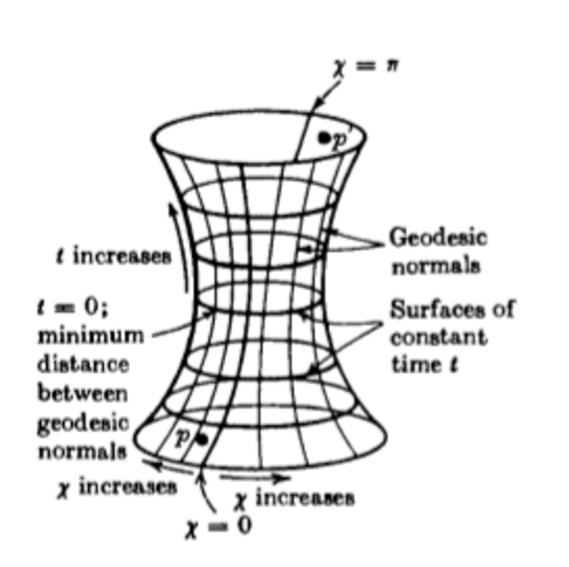
\includegraphics[width=5cm,angle=0]{deSitter.pdf}
     \caption{}
    \label{desitter}
\end{center}
\end{figure}
\subsubsection{Open Chart}
次に,この章で大切になるOpen Chartについて学ぶ,Open Chartは,(\ref{1.2})式で,座標変換$(t,r,\theta,\phi)$を
\begin{eqnarray}
  x_0&=&H^{-1}\sinh{t}\cosh{r} \\
  x_1&=&H^{-1}\cosh{t} \geqslant H^{-1} \\
  x_2&=&H^{-1}\sinh{t}\sinh{r}\cos{\theta} \\
  x_3&=&H^{-1}\sinh{t}\sinh{r}\sin{\theta}\cos{\phi} \\
  x_4&=&H^{-1}\sinh{t}\sinh{r}\sin{\theta}\sin{\phi} \\
\end{eqnarray}
によって座標系を導入した場合のChartである.このChartにおける計量は,
\begin{eqnarray}
\label{openM}
      ds^2=H^{-2}\biggr[-dt^2+\sinh^2{t}(dr^2+\sinh^2r(d\theta^2+\sin^2\theta d\phi^2))\biggr]
\end{eqnarray}
となる,ここで,$dr^2+\sinh^2r(d\theta^2+\sin^2\theta d\phi^2)$の部分は,よく$dH_3^2$という表記で省略されることが多い,

中央部分ののChartの張り方,
\begin{align}
  \label{1.19}
  x_0&=H^{-1}\cos{t}\sinh{r} \\
  \label{test}
  x_1&=-H^{-1}\sin{t} \\
  x_2&=H^{-1}\cos{t}\cosh{r}\cos{\theta} \\
  x_3&=H^{-1}\cos{t}\cosh{r}\sin{\theta}\cos{\phi} \\
  x_4&=H^{-1}\cos{t}\cosh{r}\sin{\theta}\sin{\phi} \\
\end{align}
を導入することで,得られる,ここで$x_1$は三角関数のみで表せれるので,取りうる値が制限されて,
\begin{align}
  -H^{-1} \leqslant x_1 \leqslant H^{-1}
\end{align}
であることから,このChartは確かに,中央の部分しか覆っていない,また,途中でChartが途切れているように見えるが,はじめのGlobal Chartで見たように,角度部分には重複があり左回りと右回りでは,どちらも$t$が増加する向きである.この座標系を導入すると,(\ref{1.2})式は,
\begin{align}
\label{CenterM}
  ds^2=H^{-2}\biggl[dt^2+\cos^2t(-dr^2+\cosh^2r(d\theta^2+d\phi^2\sin^2\theta))\biggr]
\end{align}
となる.

\subsection{Euclidean de Siiter space}
Euclidean de Sitter Spaceとは,5次元Euclid空間に埋め込めこまれた4次元球である,その超曲面は,
\begin{eqnarray}
  \tilde{x}_0^2+x_1^2+x_2^2+x_3^2+x_4^2=H^{-2}
\end{eqnarray}
で定義できる.この超曲面場での座標系は,次のように張ることができる.
\begin{eqnarray}
  \label{1.19}
  \tilde{x}_0&=&H^{-1}\cos{\tau}\cos{\rho} \\
  \label{test}
  x_1&=&H^{-1}\sin{\tau} \\
  x_2&=&H^{-1}\cos{\tau}\sin{\rho}\cos{\theta} \\
  x_3&=&H^{-1}\cos{\tau}\sin{\rho}\sin{\theta}\cos{\phi} \\
  x_4&=&H^{-1}\cos{\tau}\sin{\rho}\sin{\theta}\sin{\phi} \\
\end{eqnarray}
ただし,
\begin{eqnarray}
  \label{1.25}
  -\frac{\pi}{2} \leqslant \tau \leqslant \frac{\pi}{2},\hspace{0.5cm} 0 \leqslant \rho \leqslant \pi,\hspace{0.5cm} 0 \leqslant \theta \leqslant \pi, \hspace{0.5cm} 0 \leqslant \phi \leqslant 2\pi
\end{eqnarray}
である.5次元Eclide空間における計量は,
\begin{eqnarray}
  ds_{E}^2=d{\tilde{x}_0}^2+dx_1^2+dx_2^2+dx_3^2+dx_4^2
\end{eqnarray}
 なので,この超曲面の計量は,
 \begin{eqnarray}
   \label{4sphereM}
   {ds_{E}}^2=H^{-2}\biggl[d\tau^2 + \cos^2\tau(d\rho^2+\sin^2\rho d\Omega^2)\biggr]
 \end{eqnarray}
 という形になる.次に,この時空において,$\tilde{x}_0\rightarrow ix_{0}$のwickローテーション(analytic continuation)を行う.この操作で,多様体は3つのLorentz多様体に分けることができる.この操作について詳しくみていくことにする.(\ref{1.19})式を見れば,
 \begin{eqnarray}
   ix_0=\cos\tau\cos\rho
 \end{eqnarray}
を満たすことになる.今,座標$x_0$は,Real numberなので,左辺はimaginary numberとなることがわかる.一方,$\tau$と$\rho$が独立な変数であることに注意する\footnote{$\cos=a+ib,\cos\rho=c+id$とおいた時に,これらの積がpure imaginaryになるのは$ac-bd=0$の時である,しかし,このように$a,b,c,d$を取ると$\tau$と$\rho$が独立で無くなる},$x_0$がrealになるためには,次の2パターンが考えられる.
\begin{center}
  (i)\ $\cos\tau$がrealで$\cos\rho$がpure imaginary \\
  (ii)\ $\cos\tau$がpure imaginaryで$\cos\rho$がreal
\end{center}

それぞれの場合について,metric(\ref{4sphereM})がどのようにwick rotationされるかを考える.
ただし,三角関数と双曲線関数の関係,
\begin{eqnarray}
  \label{1.29}
  \sin{i\theta}=i\sinh{\theta} \\
  \label{1.30}
    \cos{i\theta}=\cosh{\theta}
\end{eqnarray}
と,$\rho,\tau$のwick rotationで他の変数$x_1\sim x_4$が複素数にならないようにすることに注意する.
\subsubsection{(i)}
$\cos\tau$がrealとなることから$\tau$は,realまたはimaginalのどちらかである,もし,複素数であれば,加法定理で分解した時に$\sin$の因子からimaginary numberが出てくる.また,$\tau$がpure imaginalであれば,$x_2\sim x_4$が(\ref{1.29})式からimaginary numberとなるので不適.従って,$\tau$はreal numberであれば良いことがわかった.次に$\sin\rho$がimaginary numberになるには,
\begin{eqnarray}
  \rho=\pm ir+\frac{\pi}{2}
\end{eqnarray}
と取ればいい.ただし,$\rho$の実部の取りうる範囲(\ref{1.25})に注意した.

以上より,(i)の場合は,
\begin{align}
  \tau&=t_{C} \\
  \rho &= \pm ir_{C} +\frac{\pi}{2}
\end{align}
というようにwick rotationすればいいことがわかる.
これを,$r_{C},t_{C}$についてとくと,
\begin{align}
  t_{C} = \tau& &(-\frac{\pi}{2} \leqslant t_{c} \leqslant \frac{\pi}{2}) \\
  r_{C} =i(\rho-\frac{\pi}{2})& &(-\infty \leqslant r \leqslant \infty)
\end{align}
となる,ただし,$\rho$の係数の符号は,$x_0$が正の値になるように,定めた.
この変換の下で,メトリック(\ref{4sphereM})式は,
\begin{align}
  ds^2=H^{-2}\biggl[{dt_{C}}^2+\cos^2t_{C}(-{dr_{C}}^2+\cosh^2r_{C}d\Omega^2) \biggr]
\end{align}
となる.これはちょうどde Sitter時空の中央をおおうChart(\ref{CenterM})式に一致する.
\subsubsection{(ii)}
次に,$\cos\tau$がpure imaginaryで$\cos\rho$がrealである場合について考える.
このとき,$\tau$は,次の場合にが考えられる.
\begin{align}
  \tau=it\pm\frac{\pi}{2},-it\pm\frac{\pi}{2}
\end{align}
ただし,real partが$\frac{\pi}{2}$となるように選んだ理由は,$\tau$の変域とpure imaginaryになるようにするためである,$\cos\tau$imaginary numberであるとき,$\sin\rho$がrealであれば,$x_2 \sim x_4$がimaginary numberとなるので,$\rho$は$\sin\rho$がpure imaginaryかつ,$\cos\tau$が仮定からrealになるように取ればいい.その候補として,
\begin{align}
  \rho=\pm ir
\end{align}
が考えられる.先ほど同様に,$x_0$が正の値になるようにこれらの値を定めると,
\begin{align}
  \label{1.47}
  \tau&=it-\frac{\pi}{2},-it+\frac{\pi}{2} \\
  \label{1.48}
  \rho &= \pm ir
\end{align}
まで絞られる.\footnote{wick rotationした後の$x_0$は,(\ref{1.47})を代入すると,$x_0=\cosh{r}\sinh{t}$となるが,$t \geqslant 0$に制限すれば,この値は常に正の値になる.}一方,$\rho$の符号の不定性は,$x_2\sim x_4$が正負どちらの値も取りうるので,$x_0$の場合と異なりどちらでも良いが,ここでは$x_2\sim x_4$の係数$\cos\tau\sin\rho$がはじめ正の値になるように定めると,
\begin{align}
  \cos\tau\sin\rho&=\cos(+it-\frac{\pi}{2})\sin(\pm ir) \\
  &=i(\pm i)\sinh{t}\sinh{r}
\end{align}
となるので,$\rho=-ir$と選べば良いことになる.以上より,(ii)の場合では,
\begin{align}
  \label{1.49}
  \tau&=it_{L}-\frac{\pi}{2},-it_{R}+\frac{\pi}{2} \\
  \label{1.59}
  \rho&=-ir
\end{align}
すなわち,
\begin{align}
  t_{R}&=i(\tau-\frac{\pi}{2})& &(t_{R} \geqslant 0) \\
  r_{R}&=i\rho& &(r_{R} \geqslant 0) \\
  t_{L}&=-i(\tau+\frac{\pi}{2})& &(t_{L} \geqslant 0) \\
  r_{L}&=i\rho& &(r_{L} \geqslant 0)
\end{align}
と定めれば良いことがわかる,
また,このような変換の元で,超曲面のメトリック(\ref{4sphereM})は,それぞれ,
\begin{align}
  ds^2&=H^{-2}\biggr[-dt_{R}^2+\sinh^2{t_{R}}(dr_{R}^2+\sinh^2r_{R}(d\theta^2+\sin^2\theta d\phi^2))\biggr] \\
ds^2&=H^{-2}\biggr[-dt_{L}^2+\sinh^2{t_{R}}(dr_{L}^2+\sinh^2r_{L}(d\theta^2+\sin^2\theta d\phi^2))\biggr]
\end{align}
のようになる,これらは,(\ref{openM})式で表されるOpen Chartのメトリックに一致する.また,ここでは,$\tau$の実部として$\frac{\pi}{2}$を選んだものを$R$側のChart,$-\frac{\pi}{2}$を選んだものを$L$側のChartとしている.

以上より,5次元Euclid時空に埋め込まれた,4次元球の超曲面が作る時空において第$0$成分をwick rotationすることで時空は,3つのopen chart($R,L,C$)に対応するde Sitter時空に分けられるということが結論づけられた.上の変換では,$\rho$と$\tau$をreal numberからcomplex numberへ拡張したので,単純に変数の自由度が増えているように見えるが実際は,増えていない.実際,(\ref{1.47})式では,$\tau$のreal partは,RとL領域で一意に$\pm\frac{\pi}{2}$に決まっている.また,(\ref{1.48})式に関しても,$r$は,real numberなので$\rho$はpure imaginaryで自由度が変わっていない.(\ref{1.49}),(\ref{1.50})式に関しても同様である.

最後に,R領域とL領域につながりについて考える.上で議論したように,RとLは,$\tau$が$(-\frac{\pi}{2},\frac{\pi}{2})$で変換するようなpathによって繋がっている.この時,pathとして上の議論では$x_0$が正になるようなpathについて今回は考えたが,逆の半球に関するpathでも繋がっている.(例えば,図\ref{desRL}のちょうど真ん中の線は,右のL領域の$(\rho=0,-\tau=\frac{\pi}{2})$から始まり,$(\rho=\frac{\pi}{2},-\tau=\frac{\pi}{2}\sim\frac{\pi}{2})$のCの領域を通過して,$(\rho=0,\tau=\frac{\pi}{2})$の左側R領域に到達するpathで繋がっている.)
また,中央のC領域は,$\rho~\frac{\pi}{2}$なる領域としてこの半球に加わっている.(Euclidのときにお覆えていた一部の領域は変数が一部imaginary numberになるため覆えなくなっている.)\footnote{此処までの操作で全体を覆っていた座標系($\tau,\rho,\theta,\phi$)からwick rotationを挟むことによって
一部領域が覆えなくなり,RとLは分離された別々のChartになる.一方,複素数になるので今まで覆えていなかった部分が新しく覆われることになる.}

\begin{figure}[H]
  \begin{center}
  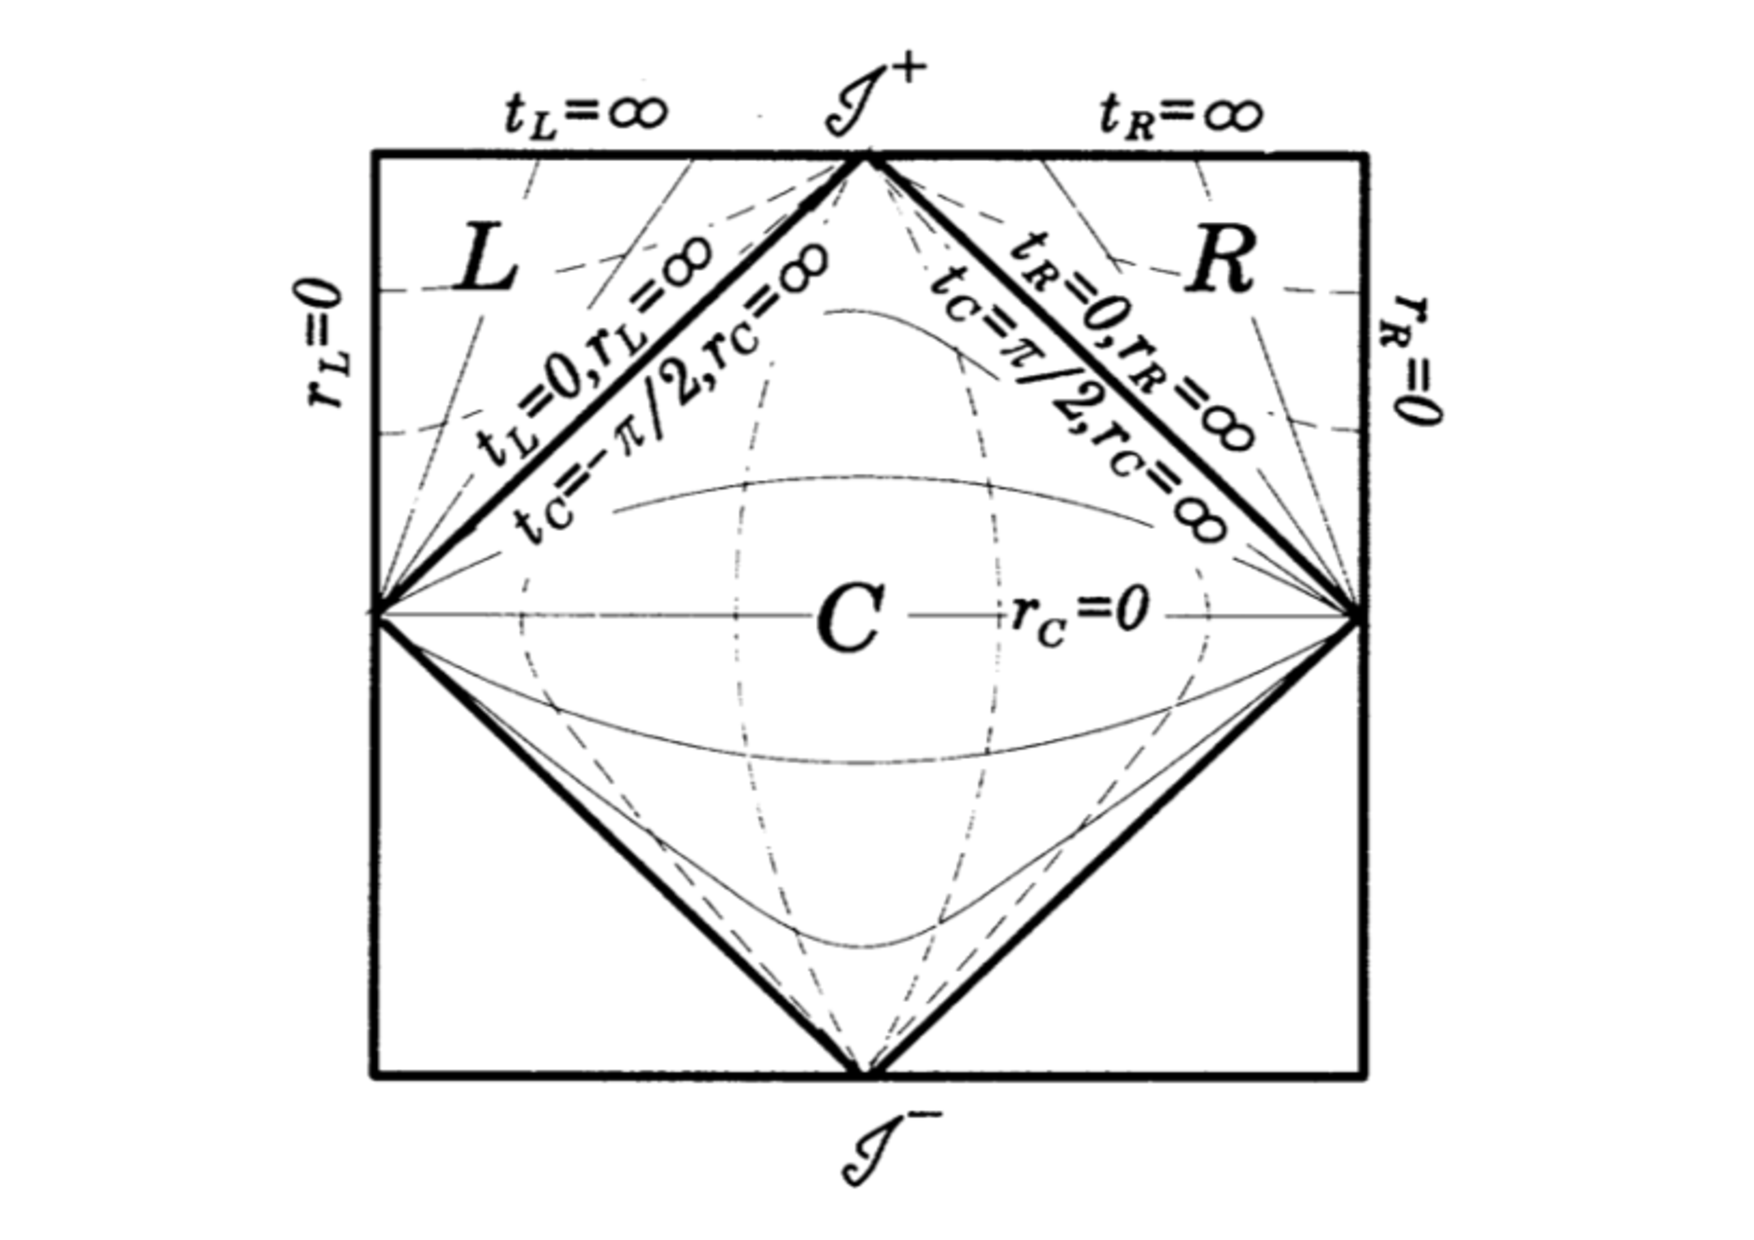
\includegraphics[width=8cm,angle=270]{desRL.pdf}
  \caption{Conformal Diagram of de Sitter space}
    \label{desRL}
  \end{center}
\end{figure}

\subsubsection{Open Chart}
\subsubsection{Scalar field on de Sitter Space}
次に,質量が$m$のfree scalar field $\varphi$について考える,lagrangianは次で与えられる,
\begin{align}
S=\int d^4x\biggr(\frac{1}{2}\sqrt{-g}(-g^{\mu\nu}\partial_{\mu}\varphi\partial_{\nu}\varphi-m^2\varphi^2-\xi R \varphi^2)\biggl)
\end{align}
ここで,今回は,作用の第三項に曲率とscalar fieldのカップリングを導入した.\footnote{\textcolor{red}{このように曲率との結合を考える正当性についてはもう少し学ぶ必要がありそう.}}また,その結合定数を$\xi$で与えた.この項は,理論上入る可能性があるが観測では曲率が0に近いので実際に必要であるかどうか難しいところである,今回は,$m_{eff}^2=m^2+\xi R$のように有効質量を用いることで普段と同様の扱いができることを利用して考える.ちなみに,de Sitter時空におけるRicci scalarは,
\begin{align}
  R=12H^{-2}
\end{align}
であるので,lagrangianは,
\begin{align}
  \label{1.60}
  \mathcal{L}&=\frac{1}{2}\sqrt{-g}(-g^{\mu\nu}\partial_{\mu}\varphi\partial_{\nu}\varphi-m^2\varphi^2-12H^{-2}\xi \varphi^2) \\
  \label{1.61}
  &=\frac{1}{2}\sqrt{-g}(-g^{\mu\nu}\partial_{\mu}\varphi\partial_{\nu}\varphi-m_{eff}^2\varphi^2)
\end{align}
とかける,ただし,有効質量は,
\begin{align}
  m_{eff}^2=m^2+12H^{-2}\xi
\end{align}
で定義した.このときの運動方程式は,EL方程式(\ref{EL})より,
\begin{align}
    \frac{1}{\sqrt{-g}}\partial_{\mu}\biggl(\sqrt{-g}g^{\mu\nu}\partial_{\nu}\varphi
\biggr)
    -m_{eff}^2\varphi=0
\end{align}
となる,ここで,Padmanの(4.108)式にあるように,
\begin{align}
  \label{1.65}
  \nabla_{\mu}\nabla^{\mu}\varphi=\frac{1}{\sqrt{-g}}\partial_{\mu}\biggl(\sqrt{-g}g^{\mu\nu}\partial_{\nu}\varphi\biggr)
\end{align}
であるので,運動方程式は,さらにシンプルな形にまとめられて,
\begin{align}
  \label{1.66}
  \biggl[g^{\mu\nu}\nabla_{\mu}\nabla_{\nu}-m_{eff}^2\biggr]\varphi=0
\end{align}
となる,この方程式は,flatな場合のKlein-Gordon方程式を重力がある時に拡張した形になっている.(偏微分$\partial$を共変微分$\nabla$に変えた形になっている.)
次に,$\varphi$をRとL領域においてモード展開する.場の演算子$\varphi$は,(\ref{1.66})式の解(固有関数モード)の線形結合で表されるので,
\begin{align}
  \varphi(t,r,\Omega)=\sum_{\Lambda}(\hat{\bm{a}}_{\Lambda}u_{\Lambda}(t,r,\Omega)+\hat{\bm{a}}^{\dagger}_{\Lambda}u^{*}_{\Lambda}(t,r,\Omega))
\end{align}
と展開できる.ただし,$u_{\Lambda}(t,r,\Omega)$は,(\ref{1.66})式を満たす固有関数である,
\begin{align}
  \label{1.68}
\biggl[g^{\mu\nu}\nabla_{\mu}\nabla_{\nu}-m_{eff}^2\biggr]u_{\Lambda}(t,r,\Omega)=0
\end{align}
この関数,すなわちopen chartのEuclidean vacuum におけるモード関数を求めるために,(\ref{1.68})式を$g^{\mu\nu}$が$g_{\mu\nu}$の逆行列であることに注意して,$(t,r,\Omega)$を用いて書き下すと,(具体的には,(\ref{1.65})式を用いて書き出すほうが楽である.ここで,$\sqrt{-g}=H^{-4}\sinh^3t\sinh^2r\sin\theta$であることを用いた.)
\begin{align}
  \biggl[\frac{1}{\sinh^3t}\frac{\partial}{\partial t}\sinh^3t\frac{\partial}{\partial t}-\frac{1}{\sinh^2t}\bm{L}^2_{H^3}+\frac{4}{9}-\nu^2\biggr]u(t,r,\Omega)=0
\end{align}
となる.この方程式はR,Lのそれぞれの領域で成り立つ.したがって,$(t,r)=(t_{R},r_{R}) or (t_{L},r_{L})$である,
また,ラプラシアン$L_{H^3}^2$と$\nu$はそれぞれ,
\begin{align}
  \bm{L}_{H^3}^2&=\frac{1}{\sinh^2r}\frac{\partial}{\partial r}\biggl(\sinh^2r\frac{\partial}{\partial r}\biggr)+\frac{1}{\sinh^2r}\bm{L}_{\Omega}^2 \\
  \bm{L}_{\Omega}^2&=\frac{1}{\sin\theta}\frac{\partial}{\partial \theta}\sin{\theta}\frac{\partial}{\partial \theta}+\frac{1}{\sin^2{\theta}}
  \frac{\partial^2}{\partial \phi^2} \\
  \nu&=\sqrt{\frac{9}{4}-\frac{m^2_{eff}}{H^{2}}}
\end{align}
で表される.Lagragianがローレンツ変換に対する対称性があるので,RとLは完全に対称な形で運動方程式が与えられる.次に,モード関数$u_{\Lambda}(t,r,\Omega)$を$t$に関係する部分とそれ以外に分離する.
\begin{align}
  u_{\Lambda}(t,r,\Omega)&=\chi(t)Y_{plm}(r,\Omega)\\
  &=\chi(t)f_{pl}(r)Y_{lm}(\theta,\phi)
 \end{align}
 \textcolor{red}{この変数分離で表せない解はないのか}
このとき,$\bm{L_{\omega}^2}$部分は,固有値方程式,
\begin{align}
  L_{\Omega}^2Y_{lm}(\theta,\phi)=-l(l+1)Y_{lm}(\theta,\phi)
\end{align}
を満たし,固有値$l,m$によって特徴付けられる,(右辺の符号がマイナスであれば,この方程式は,ルジャンドルの陪微分方程式になる.)
また,$Y_{plm}(r,\Omega)$の部分は,\textcolor{red}{あとで確認するように,次の固有値方程式を満たすことがわかる.}
\begin{align}
  \bm{L}_{H^3}^2Y_{plm}(r,\Omega)&=-(1+p^2)Y_{plm}(r,\Omega) \\
  &or \\
 \bm{L}_{H^3}^2f_{pl}(r)Y_{lm}(\theta,\phi)&=-(1+p^2)f_{pl}(r)Y_{lm}(\theta,\phi)
\end{align}
そこでこれを,具体的に書き下すと
\begin{align}
\biggl(\frac{1}{\sinh^2r}\frac{\partial}{\partial r}\biggl(\sinh^2r\frac{\partial}{\partial r}\biggr)+\frac{1}{\sinh^2r}\bm{L}_{\Omega}^2\biggr)f_{pl}(r)Y_{lm}(\theta,\phi)=-(1+p^2)Y_{plm} \\
\label{1.80}
\therefore\biggl(\frac{1}{\sinh^2r}\frac{\partial}{\partial r}\biggl(\sinh^2r\frac{\partial}{\partial r}\biggr)-\frac{l(l+1)}{\sinh^2r}+(1+p^2)\biggr)f_{pl}(r)Y_{lm}(\theta,\phi)=0
\end{align}
ここで,$\xi=\cosh r$の座標変換をすれば,
\begin{align}
  \sinh r=\xi^2 -1, \hspace{4mm} \frac{\partial}{\partial r}=\frac{\partial \xi}{\partial r}\frac{\partial}{\partial \xi}=\sinh r\frac{\partial}{\partial \xi}
\end{align}
であるので,(\ref{1.80})式は,
\begin{align}
  \label{1.81}
\left(\left(\xi^2-1\right)\frac{\partial^2}{\partial \xi^2}+3 x \frac{\partial}{\partial \xi}-\frac{l (l+1)}{\xi^2-1}+(p^2+1)\right)f_{pl}(\xi)=0
\end{align}
のように書き換えられる.\footnote{ここまでの操作をまとめる.運動方程式は,4つの文字を含んだ偏微分方程式でむずかしいので,段階を分けて処理した.はじめに$\phi$について解き(固有値は$m$)次に,$\theta$についてといて(固有値は$l$)最後に,$r$について式を整理した.$r$だけの方程式になったのが,(\ref{1.80})式でありこれをとけば良い.}

この解は,\begin{align}
  f^l_p(\xi)=\frac{c_1 P_{i p-\frac{1}{2}}^{l+\frac{1}{2}}(\xi)+c_2 Q_{i p-\frac{1}{2}}^{l+\frac{1}{2}}(\xi)}{\sqrt[4]{\xi^2-1}}
\end{align}
となる.ここで,$P^{\mu}_{\nu}$は第1種ルジャンドルの陪関数であり,$Q^{\mu}_{\nu}$は第2種ルジャンドルの陪関数である.

ただし,$Q(\xi)$は$\xi=1$で正則でないので,$c_2=0$で落とせば,
\begin{align}
  f^l_p(\xi)=\frac{1}{\sqrt[4]{x^2-1}}c_1 P_{i p-\frac{1}{2}}^{l+\frac{1}{2}}(\xi)
\end{align}
\textcolor{red}{この解は,分母に$0$になる可能性がある因子があるので,それについてテェックしておく必要がある.
また,カシミア演算子やlorents gruopの話,固有値が$(1+p^2)$になる理由について確認する必要あり.また,Lugendre関数の初期条件or境界条件はどうしているのか}
